\Block{Introduction}{

\textbf{Motivation}

\begin{itemize}
    \item Earth's mantle, between the crust and the liquid outer core, undergoes a process known as mantle convection. A paramount challenge in essence's is reconstructing the thermochemical evolution of Earth's mantle and its various surface manifestations, where the insights into previous mantle states are imperative.

    \item Therefore, the concept of the inverse problem is introduced, whose predominant strategy is called adjoint method. Nevertheless, this approach is computationally intensive.

    \item The primary motivation behind this research is to curtail computational requirements. This is achieved by exploring the potential of deep learning methods as surrogate models that offer the means to approximate the forward and adjoint problems with significantly reduced computational cost.

    \item As a first attempt in this direction, we have addressed the forward problem associated with two well-established geodynamics problems: the `geoid' problem and the 2D Mantle convection problems.
\end{itemize}



\textbf{Geoid Problem}

\begin{figure}[H]
    \centering
    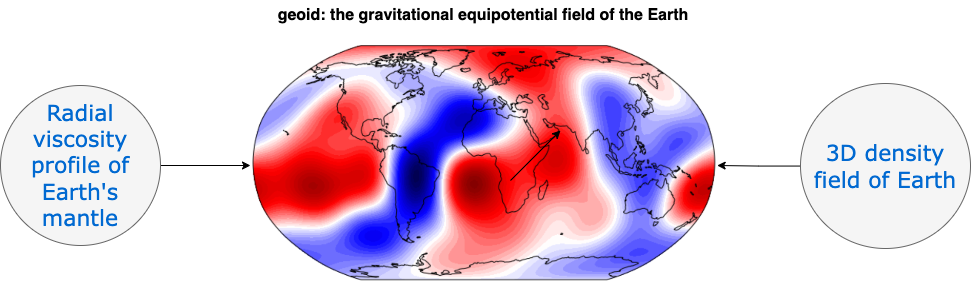
\includegraphics[width=0.8\linewidth]{figures/Geoid.png}
    \caption{Geoid and its two related factors [1].}
\end{figure}
\vspace{-2ex}
\begin{itemize}
     \item Research shows that when geoid is modelled purely based on density variation near the surface, the result can poorly explain the observed geoid measurements [1]. 

     \item Therefore, we explore the usage of Earth's viscosity to model the geoid.
\end{itemize}

\textbf{Mantle Convection Problem}

\begin{figure}[H]
    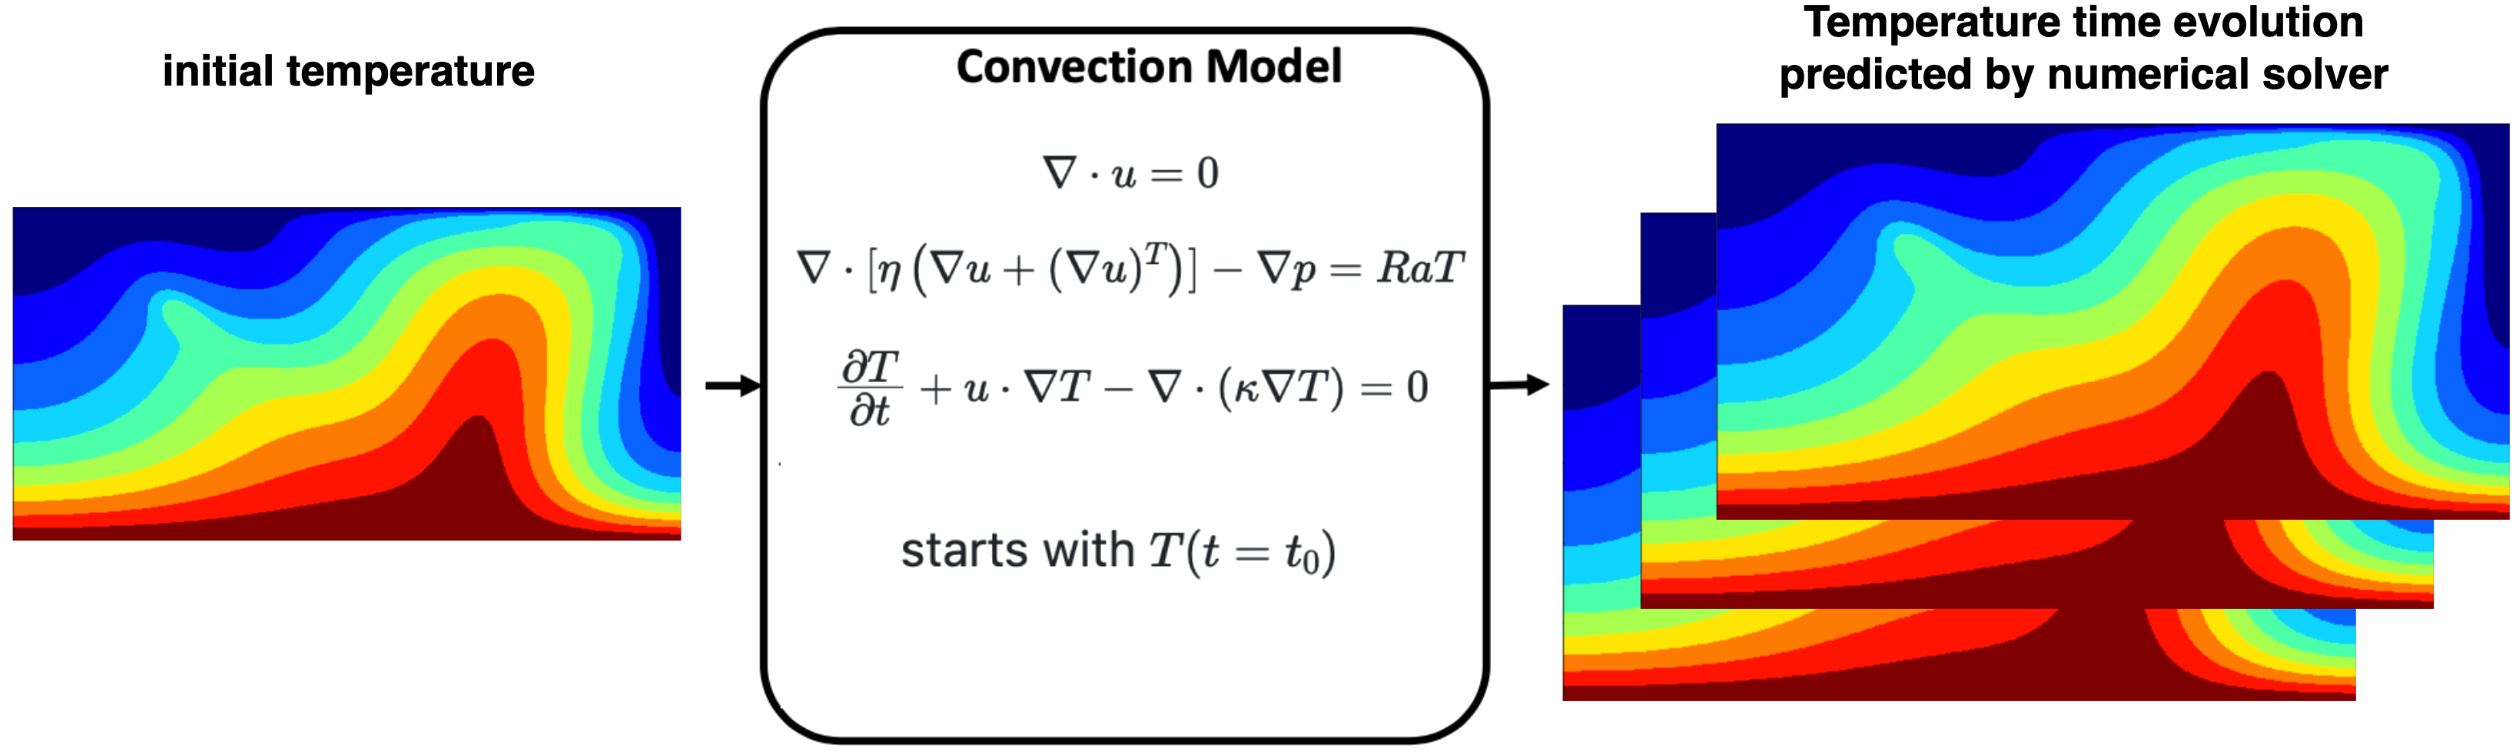
\includegraphics[width=\linewidth]{figures/Mantle_Convection_workflow.png}
    \caption{Typical mantle convection workflow.}
\end{figure}
\vspace{-2ex}
\begin{itemize}
    \item The thermal evolution is modelled using the Stokes system of partial differential equations derived from the conservation equations of mass, momentum, and energy, in their simplest form of the Boussinesq approximation. 
\end{itemize}

\textbf{Neural Networks}
\begin{itemize}
    \item Fully Connected Neural Network (FNN)
            \begin{itemize} 
                \item A parameterized function, here denoted $\mathcal{N}(\theta)$, and defined as the chained composition of $n$ affine maps $\Theta_i$ (i.e., $n$ hidden layers) and activation function $g$:
            \begin{equation*}
            \mathcal{N}(\theta) = \Theta_n \circ g \circ \Theta_{n-1} \circ \ldots \circ g \circ \Theta_1,
            \end{equation*}
            where $\theta$ represents the set of all trainable parameters.
               \item The affine maps are defined as:
		       \begin{equation*} \Theta_i(x) = xA_i^{T} + b_i, \ \mathrm{with} \ i=1,\ldots,n, \end{equation*}
            where $A_i$ and $b_i$ are the weight matrix and bias vector, respectively, corresponding to the $i$-th hidden layer.
        \end{itemize}

    \item Convolutional Autoencoders (ConvAE)
        \begin{itemize}
            \item An encoder using convolution operation to reduce the size of the original input field and output a latent space representation.

            \item A decoder using deconvolution operation to transform the latent space representation back to the original size field.
        \end{itemize}
    \item Long short-term memory (LSTM)
        \begin{itemize}
            \item Use a sequence of input recurrently to predict a sequence of output.

            \item Handle time-series data more accurately than other networks.
        \end{itemize}

\end{itemize}
}


\Block{Research Aims}{
\textbf{Geoid Problem}

\begin{itemize}
     \item To explore the usage of Neural Networks as a way to forward model the geoid problem, assuming that viscosity varying in the radial direction with depth is the most important factor.
\end{itemize}

\textbf{Mantle Convection Problem}

\begin{itemize}
    \item To explore the usage of Neural Networks as surrogate models for the original mantle convection numerical solver to significantly reduce the computational cost.
\end{itemize}
}


\Block{Methods}{

\begin{itemize}
\item Previous works have explored the usage of Convolutional Neural Networks (CNNs) to solve the inverse geoid problem directly [2] or FNNs/LSTMs to approximate the forward mantle convention problem [3]. 
\item In contrast to these works:
	 \begin{itemize}
          \item We use FNN on 1D spherically symmetric viscosity model to solve the forward geoid problem as a first step to solve the inverse geoid problem. 
          \item We aim to produce the complete mantle convection time-series from an initial temperature field, rather than the next time-step out of the previous ones for a given set of parameters of the mantle convection model.
        \end{itemize}
\end{itemize}

\bigbreak

\textbf{Geoid Problem}.
\begin{itemize}
    \item Testing on a simplified small dataset (having 1000 pairs of input and output) using a reduced prior such that the perturbations to the output are smaller.

        \begin{itemize}
            \item Input: a vector with 257 values indicating a 1D spherically symmetric viscosity model.

	    \item Output: a vector with 60 values         representing a set of spherical harmonic      coefficients describing the geoid height      on the surface of the Earth.
        \end{itemize}
\end{itemize}

\begin{figure}[H]
    \centering
    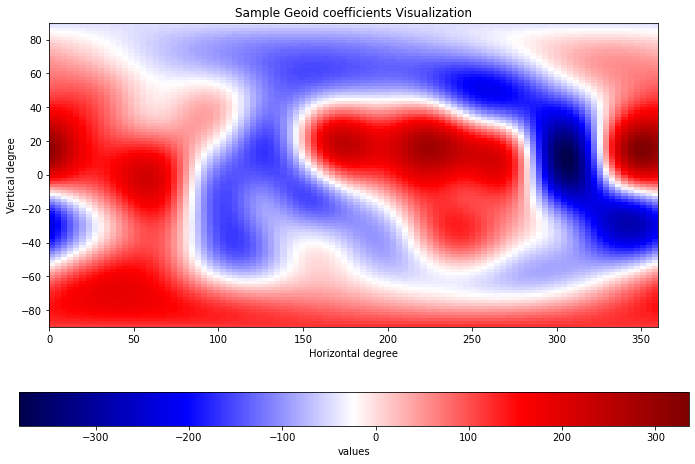
\includegraphics[width=0.5\linewidth]{figures/Geoid_Sample_visualization.png}
    \caption{Sample geoid field, where the units of the geoid are in metres and represent values greater or less than some reference value.}
\end{figure}
}



\Block{Methods (Continue)}{

\begin{itemize}
    \item Using Fully Connected Neural Networks (FNN) for prediction.

    \item Systematically training and testing different FNN architectures.
\end{itemize}

\textbf{Mantle Convection Problem}

\begin{figure}[H]
    \centering
    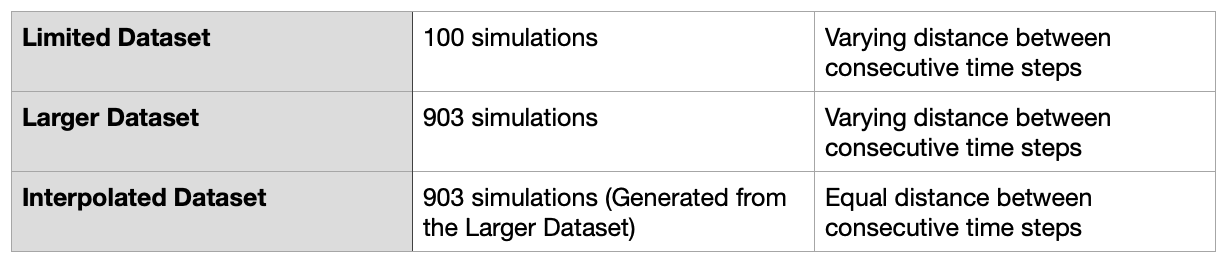
\includegraphics[width=\linewidth]{figures/Mantle_Convection_Dataset.png}
    \caption{Datasets for testing.}
\end{figure}

\begin{figure}[H]
    \centering
    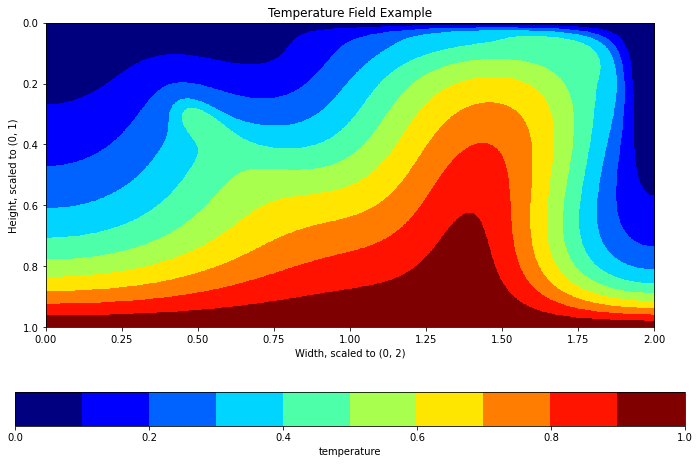
\includegraphics[width=0.5\linewidth]{figures/temperature_field_example.png}
    \caption{Sample Temperature field from datasets with size $201 \times 401$.}
\end{figure}

\begin{itemize}

    \item Using Convolutional Autoencoders (ConvAE) to compress the data into its latent space representation.
\end{itemize}

\begin{figure}[H]
    \centering
    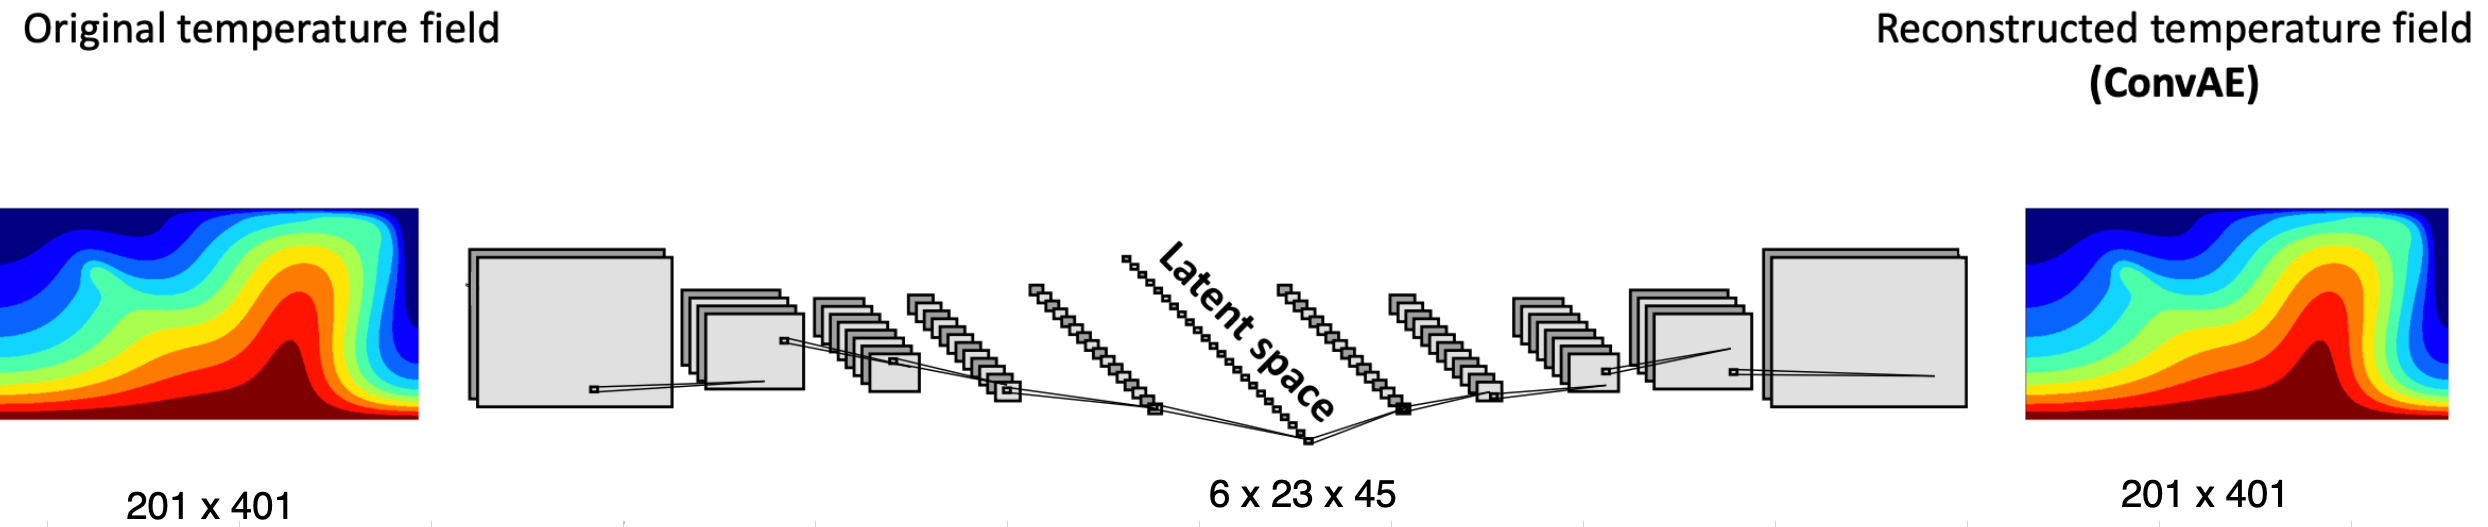
\includegraphics[width=0.8\linewidth]{figures/ConvAE_workflow.png}
    \caption{ConvAE workflow.}
\end{figure}

\begin{itemize}
    \item Given a temperature field in its latent space representation, using Fully Connected Neural Network (FNN) to predict temperature field at the next timestamp.
\end{itemize}

\begin{figure}[H]
    \centering
    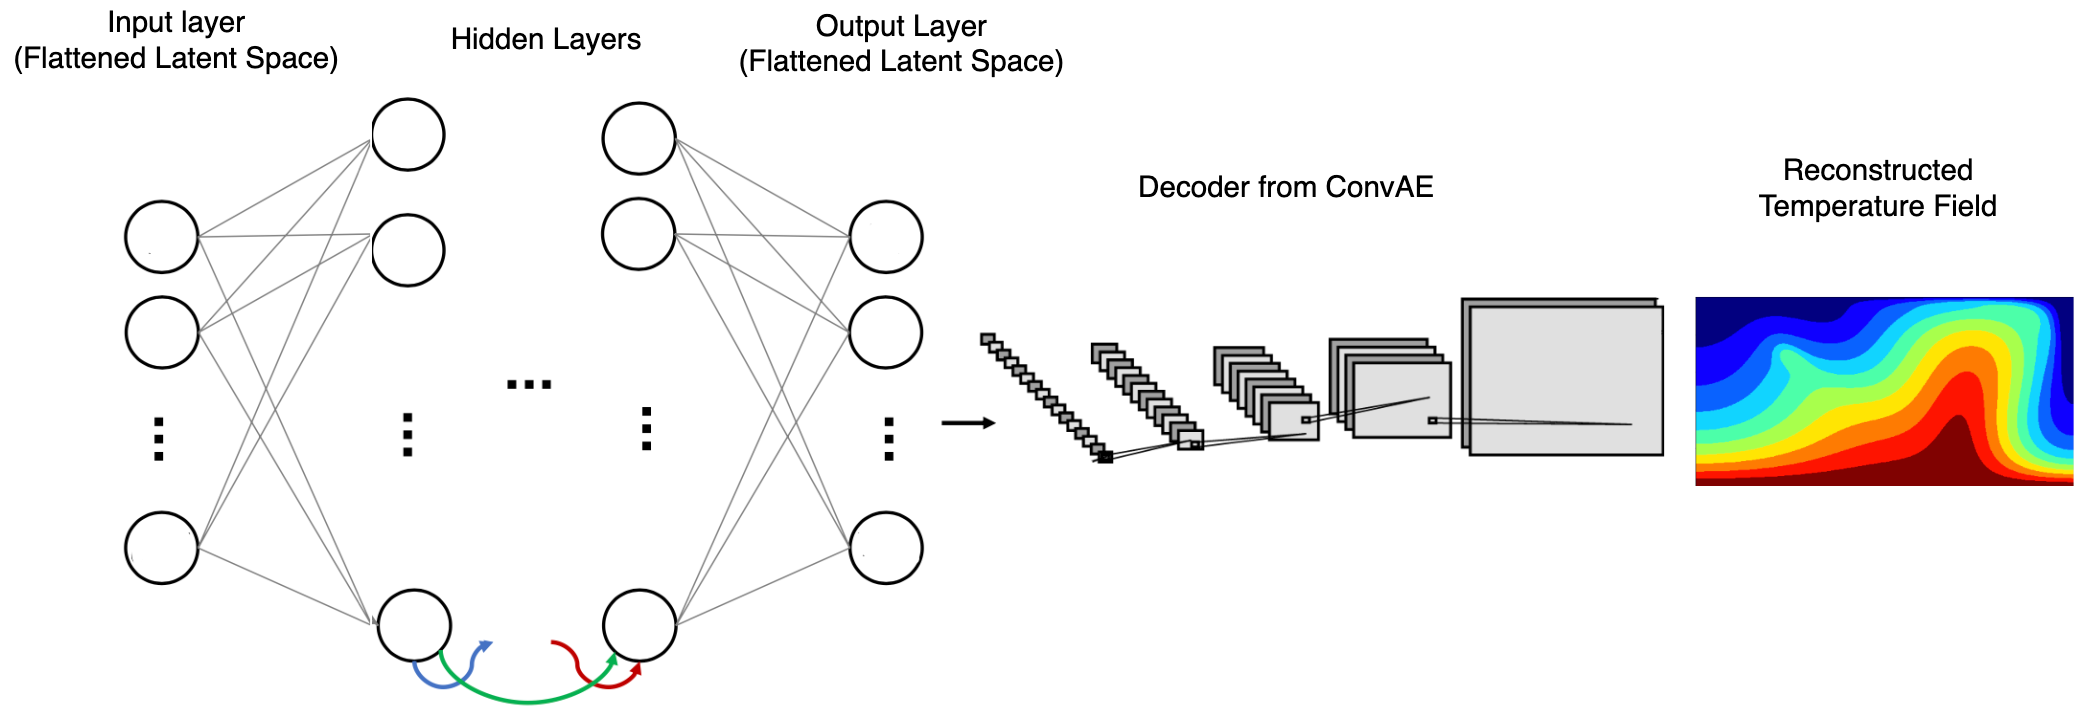
\includegraphics[width=0.8\linewidth]{figures/FNN_workflow.png}
    \caption{FNN workflow.}
\end{figure}

\begin{itemize}
    \item Two possible ways to predict a complete simulation using FNN:

        \begin{itemize}
            \item One-for-All: use $T1$ from data set $\rightarrow$ get predicted $T2$ $\rightarrow$ use predicted $T2$ $\rightarrow$ get predicted $T3$ $\rightarrow$ ...

            \item One-for-One: use $T1$ from data set $\rightarrow$ get predicted $T2$ $\rightarrow$ use $T2$ from data set $\rightarrow$ get predicted $T3$ $\rightarrow$ ...
        \end{itemize}

    \item Given the first 50 temperature fields from a simulation in its latent space representation, using Long Short-Term Memory (LSTM) to predict the last 50 temperature fields as a sequence.

\end{itemize}

\begin{figure}[H]
    \centering
    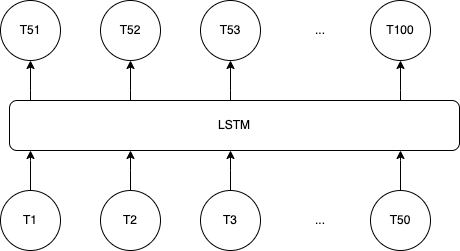
\includegraphics[width=0.8\linewidth]{figures/LSTM_workflow.png}
    \caption{General LSTM structure and the workflow in this research. (Source of the left figure: StackOverflow.)}
\end{figure}
}

\Block{Results and Findings}{

\textbf{Geoid Problem}.

\begin{itemize}
    \item FNN architectures with a total number of 4 hidden layers have the best performance (among those tested)
    when the output data is normalised using a scaler before training and testing.
\end{itemize}

\begin{figure}[H]
    \centering
    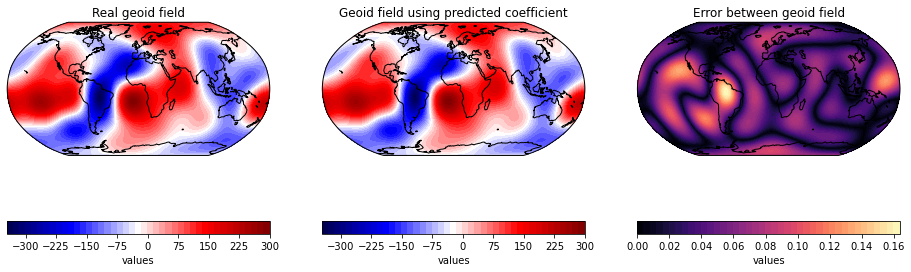
\includegraphics[width=0.8\linewidth]{figures/Geoid_Best_visualization}
    \caption{Visualization of the most accurate geoid prediction.}
\end{figure}

\begin{figure}[H]
    \centering
    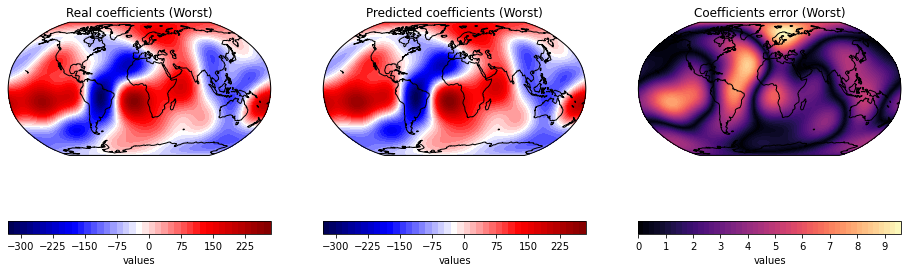
\includegraphics[width=0.8\linewidth]{figures/Geoid_Worst_visualization}
    \caption{Visualization of the least accurate geoid prediction.}
\end{figure}


\textbf{Mantle Convection Problem}

\begin{figure}[H]
    \centering
    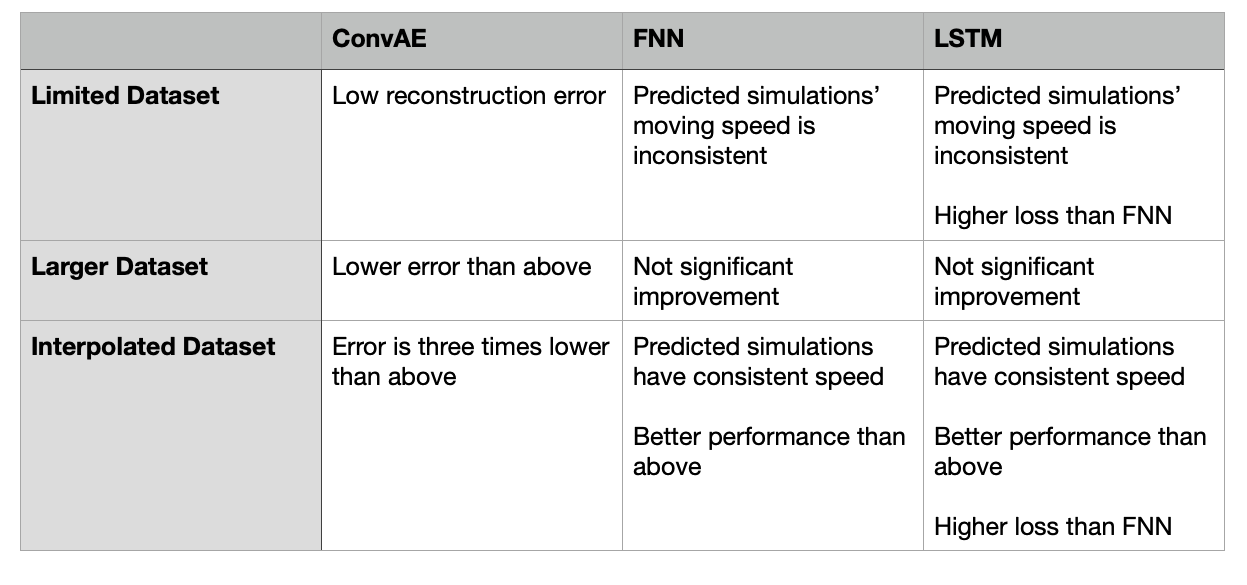
\includegraphics[width=0.9\linewidth]{figures/Mantle_Convection_Result.png}
    \caption{Testing result for three datasets.}
\end{figure}

}

\Block{Results and Findings (Continue)}{

\begin{figure}[H]
    \centering
    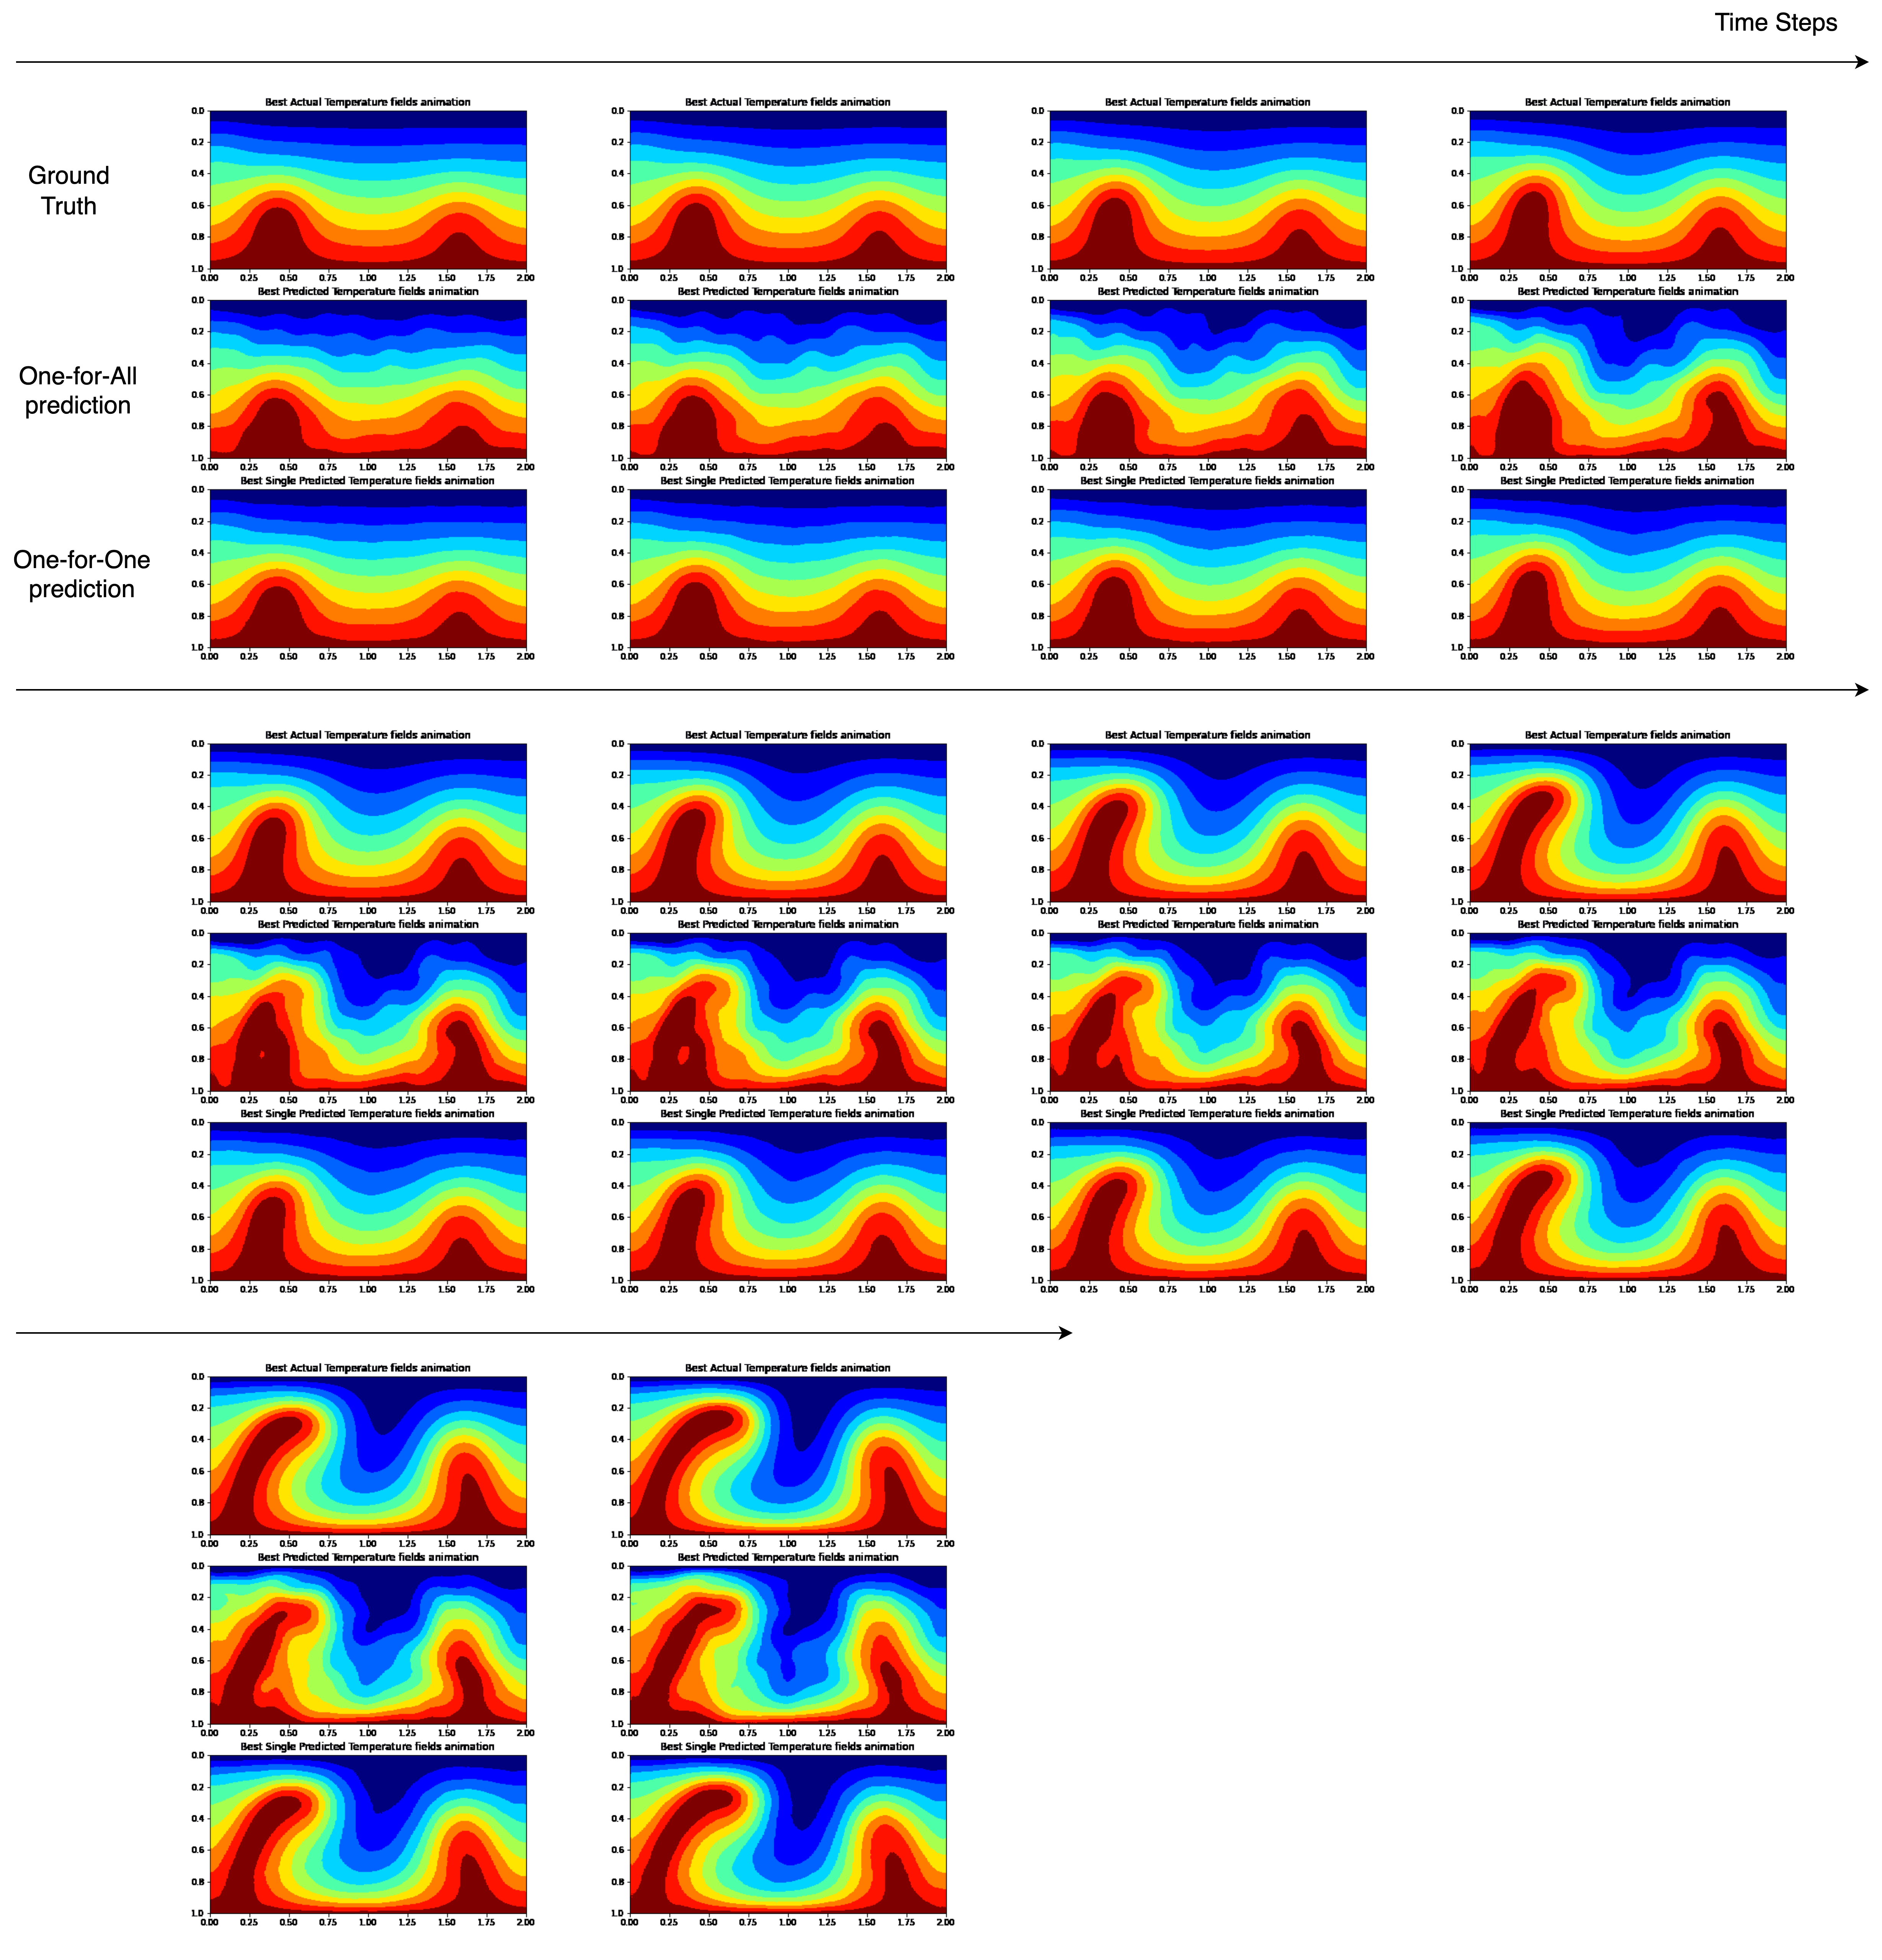
\includegraphics[width=0.9\linewidth]{figures/FNN_animation_sheet.png}
    \caption{Best case animation sheet for FNN trained with Interpolated Dataset. Predictions from 10 different time steps are presented, including 10, 20, 30, 40, 50, 60, 70, 80, 90, and 100. (see Fig. 4 for colorbar)}
\end{figure}

\begin{itemize}
    \item Further Testings on FNN trained with Interpolated Dataset
        \begin{itemize}
            \item The aim is to determine experimentally for how many time steps we can use the trained FNN during a set of S consecutive time steps (e.g., S=2 and then ”correct” the time series with the truth coming from the simulator) without losing track of the transient dynamics.
        \end{itemize}
\end{itemize}

\begin{figure}[H]
    \centering
    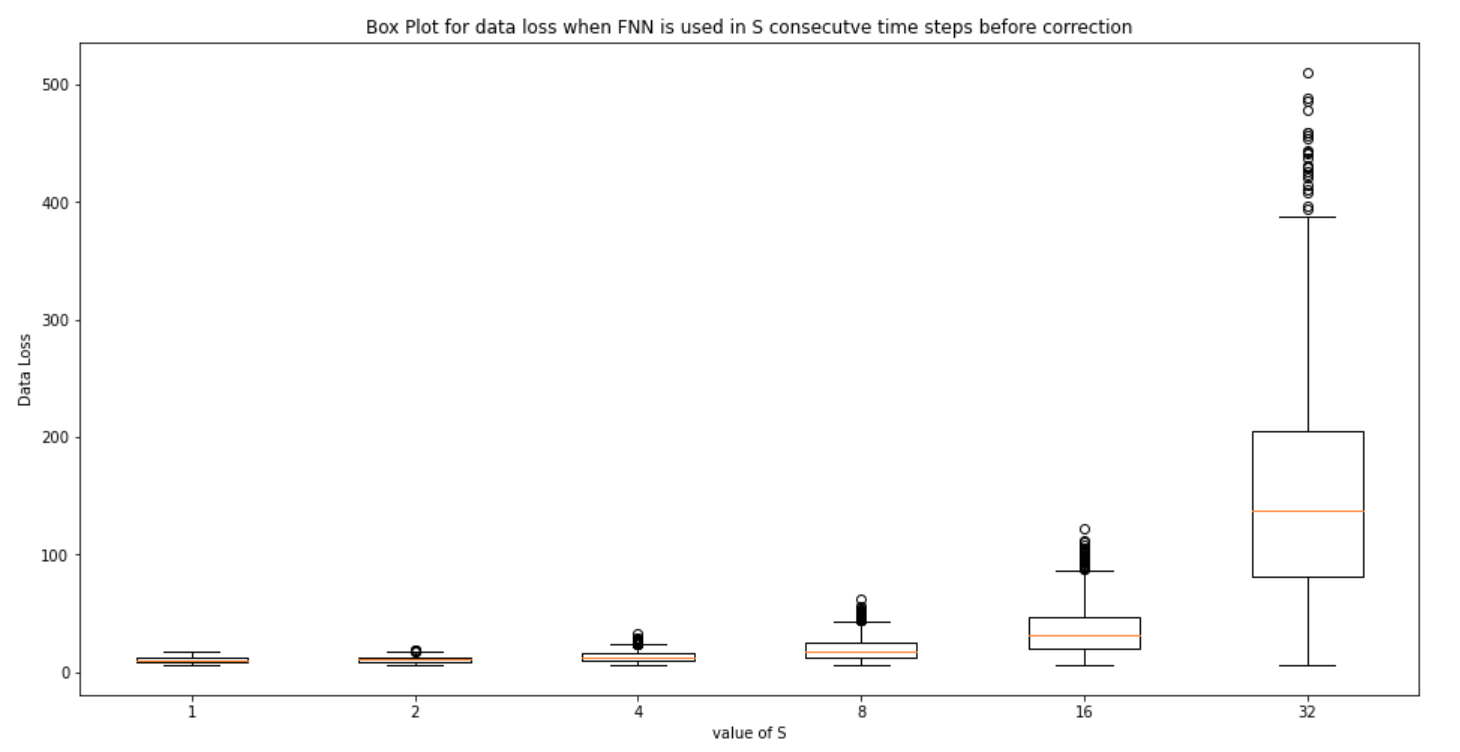
\includegraphics[width=0.8\linewidth]{figures/FNN_boxplot.png}
    \caption{Box Plot for data loss when FNN is used in S consecutive time steps before correction.}
\end{figure}

\begin{figure}[H]
    \centering
    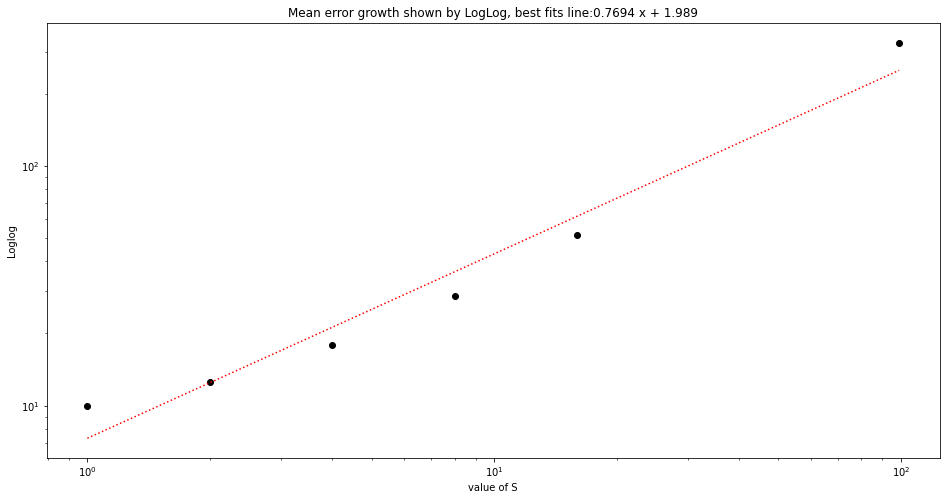
\includegraphics[width=0.7\linewidth]{figures/FNN_LogLog.png}
    \caption{Growth of average data loss with respect to the value of S shown by LogLog, which is approximately $O(0.77S)$}
\end{figure}

\begin{figure}[H]
    \centering
    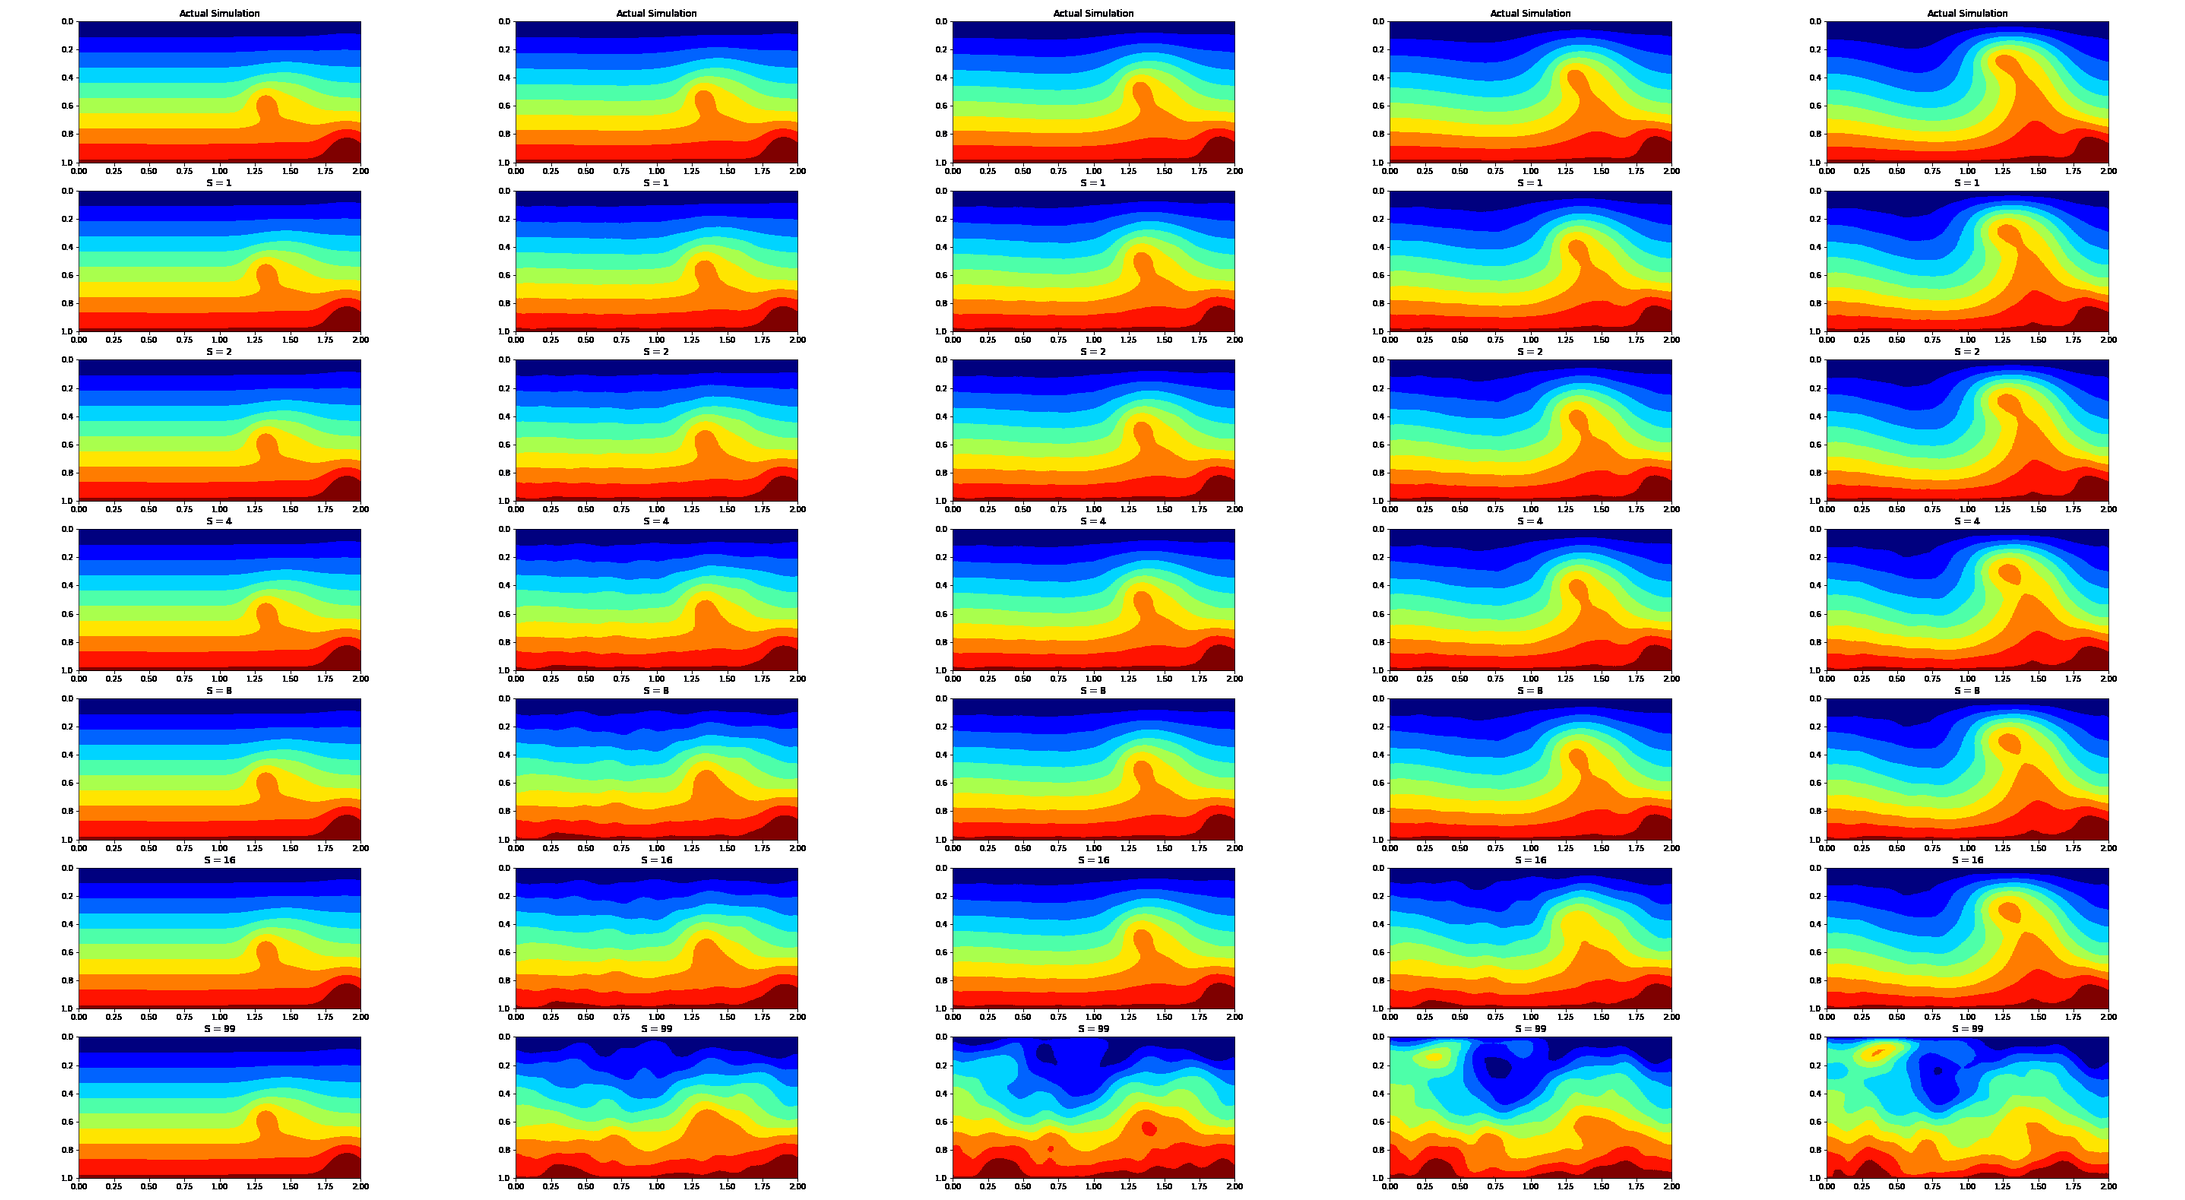
\includegraphics[width=0.9\linewidth]{figures/FNN_further_testing_sheet.png}
    \caption{Animation sheet when FNN is used in S consecutive time steps before correction, where S = 1, 2, 4, 8, 16, and 99. The time steps, from left to right, are 1, 25, 50, 75, and 100. (see Fig. 4 for colorbar)}
\end{figure}
}

\Block{Conclusion}{
\textbf{Geoid Problem}

\begin{itemize}
     \item We showed that high-dimensional regression algorithms like neural networks can help with the forward modelling of the geoid problem when predicting a set of spherical harmonic coefficients given a reduced dataset with a fairly small number of 1D spherically symmetric viscosity models.
\end{itemize}

\textbf{Mantle Convection Problem}

\begin{itemize}
     \item We use neural networks as surrogate models for mantle convection simulations and found that while the fully connected neural network (FNN) offers a better accuracy and the result has less data loss when predicting a single temperature field, the Long short-term memory (LSTM) is slightly more capable to capture the general characteristics of a complete simulation when predicting a sequence of temperature fields, compared with the One-for-All method when predicting a sequence using FNN. 

    \item We found that when FNN is used in S consecutive time steps, the growth of the data loss with S (ranging from 1, 2, 4, 8 to 16) is remarkably moderate (less than $O(S)$), with only a few outliers deviating moderately from the median. This could provide some avenues for the future research.
\end{itemize}

}

\textbf{Acknowledgements}:
This work was supported by computational resources provided by the Australian Government through the National Computational Infrastructure (NCI) under the ANU Merit Allocation Scheme.

\bigbreak

\textbf{References}:

[1] Hager, B. H., 1982. The geoid and geodynamics. Nature, 299, 5879 (sep 1982), 104–105. doi:10.1038/299104a0.

[2] Kerl, J., 2022. Geoid Inversion For Mantle Viscosity With Convolutional Neural Networks. Master thesis.

[3] Agarwal, S.; Tosi, N.; Kessel, P.; Breuer, D.; and Montavon, G., 2021. Deep learning for surrogate modeling of two-dimensional mantle convection. Physical Review Fluids, 6, 11 (nov 2021). doi:10.1103/physrevfluids.6.113801.
